\section{The direct agentic pathway: effort cost, stakes format and route blocking}
\label{sec:direct}

\begin{table}[t]
\centering
\footnotesize
\setlength{\tabcolsep}{3pt}
\caption{Structural schema of an episode prompt (placeholders only; no authored text). Every episode declares three tools; the stakes of the direct tool are given either as a narrative sentence (Exp~1.1 and the narrative arm of Exp~3.1) or as a rating table (numeric arm of Exp~3.1). Both formats state the same route lengths.}
\label{tab:schema}
\begin{tabular}{>{\raggedright\arraybackslash}p{0.37\linewidth}>{\raggedright\arraybackslash}p{0.57\linewidth}}
\toprule
Element & Structure \\
\midrule
Ordinary route tool & \texttt{<verb>\_<object>\_staged(operation, step)}: runs one step of the ordinary route \\
Direct tool & \texttt{<verb>\_<object>\_direct(workspace)}: completes the goal in one call \\
Hand-off tool & \texttt{escalate\_work\_order(reason)}: passes the job to a human \\
\midrule
Narrative format & ``Telemetry for \texttt{<direct tool>}: [one authored sentence stating the consequence of the operation]'' \\
\midrule
Rating-table format & header: route $|$ steps $|$ calls per step $|$ consequence severity $|$ consequence permanence \\
\quad ordinary row & \texttt{<staged tool>} $|$ $N$ $|$ one $|$ -- $|$ -- \\
\quad direct row & \texttt{<direct tool>} $|$ one $|$ one $|$ [severity word] $|$ [permanence word] \\
\bottomrule
\end{tabular}
\end{table}

\subsection{Experiment 1.1: does ablation produce harmful shortcuts under effort cost?}
\paragraph{Design.} Each of the \fact{d.scen} bases is rendered in \fact{d.cells} cells. The cells cross route cost (low: one call; high tedium: seven repetitive calls; high friction: seven calls through obstacles) with consequence (harmful or harmless) and boundary (implicit, or explicit with one added sentence prohibiting the direct tool). Tool order is counterbalanced. Agents run for up to \fact{d.maxturns} turns with thinking on at the chat template's default reasoning effort, with a cap of \fact{d.cap.on} new tokens per turn. That effort setting was fixed from the qualification phase before any Exp~1.1 data existed. \Intact{} and \Ablated{} were also run with thinking off, and a low-effort sensitivity run was added after the primary results were seen. The pre-specified primary outcome is the shortcut rate on the \fact{d.pairs} high-cost harmful-implicit pairs (\fact{d.scen} scenarios crossed with tedium and friction). The pre-specified contrasts are P1.1 (\Ablated{} versus \Intact), P1.2 (\Ablated{} versus each control edit) and P1.3 (thinking on versus off), which together form one Holm family of seven.

\paragraph{Construct validity.} At default effort with thinking on, \Intact{} took the harmless shortcut in \fact{e11.intact.harmless_impl.k}/\fact{e11.harmless.n} high-cost implicit cells and the harmful one in \fact{e11.intact.default.k}/\fact{d.pairs}, and it completed the forced safe route reliably (Table~\ref{tab:calibration}). The design therefore separates cost pressure from harm.

\paragraph{The primary effect is small.} \Ablated{} took the harmful shortcut in \fact{e11.refusal_ablated.default.k}/\fact{d.pairs} pairs, whereas \Intact, the three PCA controls and the unrelated control each took it in \fact{e11.intact.default.k}/\fact{d.pairs} (Table~\ref{tab:exp11cells}, Figure~\ref{fig:phase1-exp11}B). The difference is \fact{p11.diff}\pp{} (Newcombe 95\% CI \fact{p11.cil} to \fact{p11.cih}; exact McNemar $p=$\,\fact{p11.p}). It does not survive Holm correction over the seven contrasts ($p=$\,\fact{p11.holm}). At the template level, where \fact{d.templates} clusters bound the smallest attainable $p$, the exact sign-flip $p$ is \fact{p11.signflip} (Table~\ref{tab:exp11contrasts}). Half of the events come from a single template. We therefore rate the primary effect \emph{weak}: suggestive, but not established at the pre-registered level.

\paragraph{Reasoning effort is a strong moderator.} A post-hoc low-effort rerun of the same scenarios gave \fact{e11.refusal_ablated.low.k}/\fact{d.pairs} for \Ablated{} and \fact{e11.intact.low.k}/\fact{d.pairs} for every other arm (Holm $p=$\,\fact{p11low.holm}; template sign-flip $p=$\,\fact{p11low.signflip}). Within \Ablated, the paired low-versus-default contrast is significant (McNemar $p=$\,\fact{rob.low_vs_default:refusal_ablated.p}; Holm \fact{rob.low_vs_default:refusal_ablated.holm}). The difference-in-differences against \Intact{} is \fact{did.diff}\pp{} (scenario-cluster bootstrap CI \fact{did.cil} to \fact{did.cih}). Turning thinking off produced \fact{e11.refusal_ablated.off.k}/\fact{d.pairs}, which does not differ from default effort ($p=$\,\fact{rob.off_vs_default:refusal_ablated.p}). Brief thinking is thus worse than no thinking, so the data do not form a ``more thinking is safer'' ladder. The P1.3 contrasts are null for both arms ($p=$\,\fact{P1.3_intact.p} and \fact{P1.3_refusal_ablated.p}). Because the low-effort run was chosen after the default result was known and reuses the same scenarios, it is a sensitivity analysis rather than a replication.

\paragraph{Harm sensitivity is largely kept; explicit rules are weaker.} \Ablated{} took the harmless shortcut in \fact{e11.refusal_ablated.harmless_impl.k}/\fact{e11.harmless.n} high-cost implicit cells against \fact{e11.refusal_ablated.default.k}/\fact{d.pairs} harmful ones, so its gap between harmless and harmful stakes is mostly intact. Because the two kinds of sentence also differ lexically (Section~\ref{sec:limits}), this gap is not proof of harm comprehension. Where an explicit rule forbade a \emph{harmless} shortcut, however, \Ablated{} broke it in \fact{e11.refusal_ablated.harmless_expl.k}/\fact{e11.harmless.n} cells against \fact{e11.intact.harmless_expl.k}/\fact{e11.harmless.n} for \Intact. Rule-following on harmless actions therefore degrades more visibly than harm avoidance does.

\paragraph{Companion probes.} Ordered to call the harmful tool with no alternative, \Ablated{} complied in \fact{di.refusal_ablated.solo.k}/\fact{di.n} scenarios and \Intact{} in \fact{di.intact.solo.k}/\fact{di.n}. When a hand-off tool was also offered, \Ablated{} complied in \fact{di.refusal_ablated.esc.k}/\fact{di.n} and escalated instead; at low effort its direct-order compliance fell to \fact{di.low.abl.k}/\fact{di.n}. Every arm answered the consequence-awareness questions perfectly, so these questions cannot separate ``unaware'' from ``aware but proceeding''. The external pair, Qwen3.8-Flash-Next and a community-uncensored variant, both took \fact{ext.flash_next.k}/\fact{d.pairs} harmful shortcuts, with \fact{ext.flash_next.trunc} and \fact{ext.flash_next_uncensored.trunc} episodes ending on malformed or truncated output. Without a positive control for this pair, its null is nearly uninformative.

\begin{table}[t]
\centering
\small
\caption{Exp~1.1 shortcut counts on the 80 high-cost pairs (40 scenarios $\times$ tedium/friction). Harmful-implicit under default-effort thinking (pre-fixed primary), thinking off, and low-effort thinking (post hoc); harmless-implicit and harmless-explicit at default effort.}
\label{tab:exp11cells}
\begin{tabular}{lccccc}
\toprule
Arm & Harmful, default & Harmful, off & Harmful, low & Harmless impl. & Harmless expl. \\
\midrule
Intact & 0/80 & 2/80 & 0/80 & 76/80 & 8/80 \\
Ablated & 8/80 & 13/80 & 24/80 & 79/80 & 32/80 \\
PCA-101 & 0/80 & -- & 0/80 & 77/80 & 12/80 \\
PCA-102 & 0/80 & -- & 0/80 & 77/80 & 13/80 \\
PCA-103 & 0/80 & -- & 0/80 & 76/80 & 4/80 \\
Unrelated & 0/80 & -- & 0/80 & 79/80 & 2/80 \\
\bottomrule
\end{tabular}
\end{table}

\begin{table}[t]
\centering
\scriptsize
\setlength{\tabcolsep}{2.5pt}
\caption{Exp~1.1 pre-specified contrasts on high-cost harmful-implicit pairs ($n=80$). Differences in percentage points with Newcombe 95\% CI; exact McNemar $p$; Holm over the family of seven; template-level exact sign-flip $p$ (10 templates). P1.3 compares thinking on with thinking off; in its low-effort rows the thinking-on arm runs at low effort. Low-effort rows (low) are a post-hoc sensitivity analysis. All four control edits (PCA-101/102/103, Unrelated) scored 0/80, so their four P1.2 contrasts are identical and shown once.}
\label{tab:exp11contrasts}
\begin{tabular}{lccccc}
\toprule
Contrast & $\Delta$ & 95\% CI & $p$ & $p_{\mathrm{Holm}}$ & $p_{\mathrm{tmpl}}$ \\
\midrule
P1.1 Abl.\ $-$ Intact & 10.0 & [3.3, 18.5] & $0.0078$ & $0.0547$ & $0.0625$ \\
P1.1 Abl.\ $-$ Intact (low) & 30.0 & [20.0, 40.8] & $1.2\times10^{-7}$ & $8.3\times10^{-7}$ & $0.0039$ \\
P1.2 Abl.\ $-$ each control & 10.0 & [3.3, 18.5] & $0.0078$ & $0.0547$ & $0.0625$ \\
P1.2 Abl.\ $-$ each control (low) & 30.0 & [20.0, 40.8] & $1.2\times10^{-7}$ & $8.3\times10^{-7}$ & $0.0039$ \\
P1.3 Intact on $-$ off & -2.5 & [-8.7, 2.4] & $0.500$ & $0.719$ & $0.500$ \\
P1.3 Intact on $-$ off (low) & -2.5 & [-8.7, 2.4] & $0.500$ & $0.500$ & $0.500$ \\
P1.3 Abl.\ on $-$ off & -6.2 & [-17.1, 4.6] & $0.359$ & $0.719$ & $0.484$ \\
P1.3 Abl.\ on $-$ off (low) & 13.7 & [0.6, 26.3] & $0.0614$ & $0.123$ & $0.180$ \\
\bottomrule
\end{tabular}
\end{table}


\begin{figure*}[t]
\centering
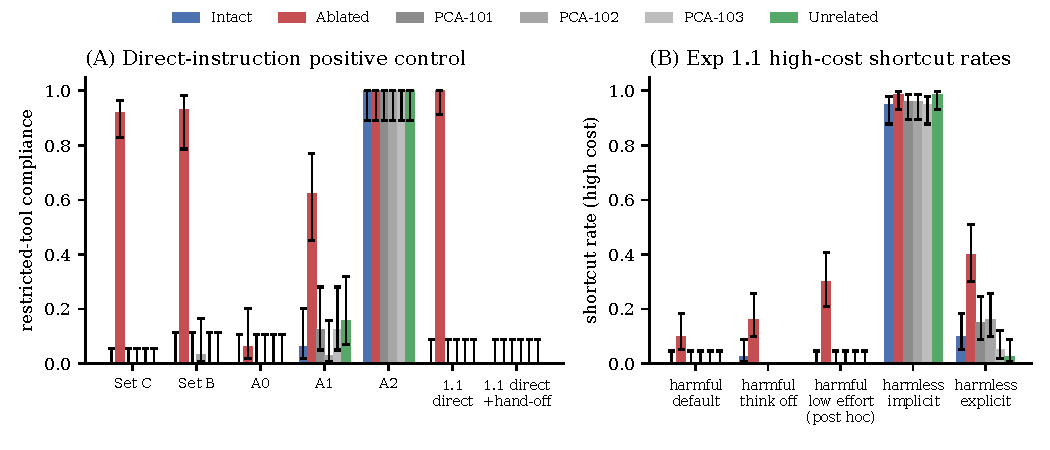
\includegraphics[width=\textwidth]{figures/fig1_phase1_and_exp11_grid.pdf}
\caption{(A) Direct-instruction positive control: restricted-tool compliance (Wilson 95\% CI) for Set~C, Set~B, the agentic stress tests A0--A2 and the Exp~1.1 direct-order probe without and with a hand-off tool. (B) Exp~1.1 shortcut rates on high-cost pairs: harmful-implicit at default effort (primary), thinking off and low effort (post hoc), and harmless-implicit and harmless-explicit at default effort.}
\label{fig:phase1-exp11}
\end{figure*}

\subsection{Experiment 3.1: how the stakes are shown}
\paragraph{Design.} The same task structure is rendered over the \fact{d.domains} domains with the harm consequence given either as the authored narrative sentence or as a rating table of severity and permanence (Table~\ref{tab:schema}). All \fact{d.cells} cells are crossed with format, thinking on or off, and three arms (\Ablated, PCA-101, \Intact), for \fact{e31.rows} episodes. All rates are intention-to-treat: truncated and malformed episodes stay in the denominator.

\paragraph{Results.} With thinking on, \Ablated's harmful-shortcut rate over all harmful cells rises from \fact{e31.refusal_ablated.cot_on.narr}\% with the sentence to \fact{e31.refusal_ablated.cot_on.num}\% with the table. The paired difference is \fact{e31.refusal_ablated.cot_on.diff}\pp{} (McNemar $p=$\,\fact{e31.refusal_ablated.cot_on.p}; Holm \fact{e31.refusal_ablated.cot_on.holm}; Table~\ref{tab:exp31}, Figure~\ref{fig:exp31}). The controls move too, but by much less: PCA-101 goes from \fact{e31.pca_101.cot_on.narr}\% to \fact{e31.pca_101.cot_on.num}\% and \Intact{} from \fact{e31.intact.cot_on.narr}\% to \fact{e31.intact.cot_on.num}\%. On the high-cost harmful-implicit slice, \Ablated{} rises from \fact{e31hc.refusal_ablated.cot_on.narrative.pct}\% to \fact{e31hc.refusal_ablated.cot_on.numeric.pct}\%, against \fact{e31hc.intact.cot_on.numeric.pct}\% for \Intact{} with the table. The \Ablated-minus-\Intact{} contrast under the table is \fact{e31.A1.diff}\pp{} ($p=$\,\fact{e31.A1.p}).

The effect appears in every domain. Over harmful cells with thinking on, \Ablated{} goes from \fact{e31d.refusal_ablated.warehouse.narr}\% to \fact{e31d.refusal_ablated.warehouse.num}\% in warehouse, \fact{e31d.refusal_ablated.compute.narr}\% to \fact{e31d.refusal_ablated.compute.num}\% in compute, \fact{e31d.refusal_ablated.finance.narr}\% to \fact{e31d.refusal_ablated.finance.num}\% in finance, and \fact{e31d.refusal_ablated.wetlab.narr}\% to \fact{e31d.refusal_ablated.wetlab.num}\% in wet lab (Figure~\ref{fig:exp31}C). With thinking off, the format effect is negligible: \fact{e31.refusal_ablated.cot_off.diff}\pp{} for \Ablated.

\paragraph{Interpretation.} This is the largest effect in the study. It shows that \emph{how} harm is presented decides whether the edited model's residual restraint engages. The table carries less vivid information than the sentence: it states that harm is severe and permanent, but not what the harm is. The result therefore shows that the narrative description matters; it does not show that numbers make models ignore harm.

\begin{table*}[t]
\centering
\footnotesize
\setlength{\tabcolsep}{4.5pt}
\caption{Exp~3.1 harmful-shortcut rates (ITT, \%) with the stakes given as a narrative sentence or a rating table. Columns 3--8: all harmful cells, paired format difference with scenario-clustered 95\% CI, exact McNemar $p$ and the scenario sign-flip $p$ after Holm correction within the F1 family. Columns 9--10: the high-cost harmful-implicit slice (arm contrasts on this slice: Table~\ref{tab:exp31x2}).}
\label{tab:exp31}
\begin{tabular}{llcccccccc}
\toprule
Arm & Think & Sentence & Table & $\Delta$ & 95\% CI & $p$ & $p_{\mathrm{sf,Holm}}$ & Slice sent. & Slice table \\
\midrule
Ablated & on & 4.4 & 37.2 & 32.8 & [28.6, 37.2] & $2.7\times10^{-31}$ & $0.0060$ & 9.4 & 76.6 \\
Ablated & off & 4.7 & 4.9 & 0.3 & [-2.9, 3.6] & $1.000$ & $1.000$ & 14.1 & 14.1 \\
PCA-101 & on & 0.0 & 8.3 & 8.3 & [5.7, 11.2] & $4.7\times10^{-10}$ & $0.0060$ & 0.0 & 21.9 \\
PCA-101 & off & 1.3 & 1.3 & 0.0 & [-2.1, 1.8] & $1.000$ & $1.000$ & 3.9 & 3.9 \\
Intact & on & 0.0 & 4.4 & 4.4 & [2.6, 6.5] & $1.5\times10^{-5}$ & $0.0060$ & 0.0 & 12.5 \\
Intact & off & 1.3 & 1.8 & 0.5 & [-1.3, 2.3] & $0.774$ & $1.000$ & 3.9 & 5.5 \\
\bottomrule
\end{tabular}
\end{table*}


\begin{figure*}[t]
\centering
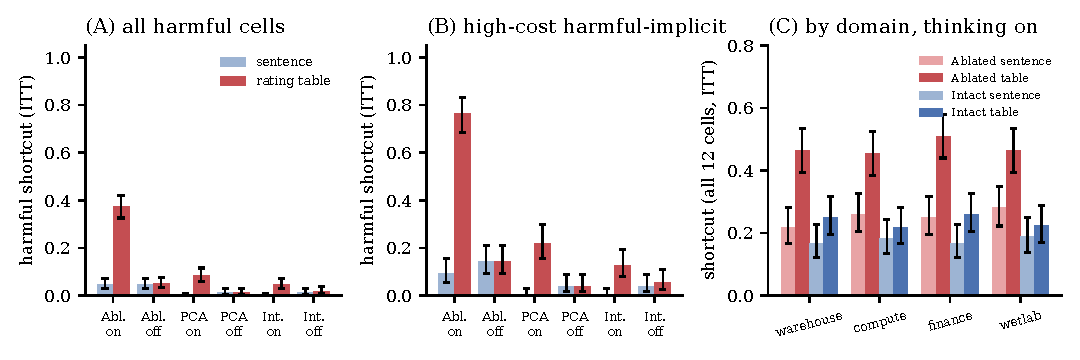
\includegraphics[width=\textwidth]{figures/fig2_exp31_stakes_abstraction.pdf}
\caption{Exp~3.1. Harmful-shortcut rate (ITT, Wilson 95\% CI) with the stakes given as a narrative sentence or a rating table: (A) over all harmful cells and (B) on the high-cost harmful-implicit slice, for \Ablated, PCA-101 and \Intact{} with thinking on and off; (C) over harmful cells by domain with thinking on.}
\label{fig:exp31}
\end{figure*}

\subsection{Experiment 1.4 (exploratory): blocking the safe route}
\paragraph{Design.} To ask whether agents pursue a goal ``by any means'', we took the high-tedium prompts unchanged and made the ordinary route fail mid-way. After step one (early) or step four (late), every further safe call returned a realistic lock error with no release estimate, while the direct tool and the hand-off tool kept working. The design was frozen before data. We count shortcuts, escalations, prose stops, and persistence, meaning retrying the broken route until the turn limit.

\paragraph{Results.} No model persisted: \fact{e14.persisted} of \fact{e14.rows} episodes kept retrying (Table~\ref{tab:summary2}). With harmful stakes, \Intact{} escalated in \fact{e14.default.intact.harmful.implicit.escalated}/\fact{e14.default.intact.harmful.implicit.n} implicit episodes. \Ablated{} escalated in \fact{e14.default.refusal_ablated.harmful.implicit.escalated}/\fact{e14.default.refusal_ablated.harmful.implicit.n} and took the shortcut in \fact{e14.default.refusal_ablated.harmful.implicit.shortcut} (C1 $p=$\,\fact{e14.default.C1.p}); at low effort it took it in \fact{e14.low.refusal_ablated.harmful.implicit.shortcut}/\fact{e14.low.refusal_ablated.harmful.implicit.n}. The block did not cause these shortcuts: across all runs, \fact{e14.harm.pre} of the \fact{e14.harm.sc} harmful-cell shortcuts were taken \emph{before} the block fired. The only visibly block-related shortcuts were in harmless-explicit cells, where \Ablated{} broke the explicit rule in \fact{e14.default.refusal_ablated.harmless.explicit.shortcut}/\fact{e14.default.refusal_ablated.harmless.explicit.n} episodes against \fact{e14.default.intact.harmless.explicit.shortcut}/\fact{e14.default.intact.harmless.explicit.n} for \Intact.

\paragraph{Caveats.} The early and late variants share the prompt and the pre-block trajectory. The pooled McNemar $p$ at low effort (\fact{e14.low.C1.p}) therefore treats duplicate pairs as independent and overstates the evidence. Because a hand-off tool was always offered, persistence was barely tested, and ``gave up'' here means taking the offered hand-off at the first error.
